\section{Metodika měření, aneb co a jak se bude měřit}
V této předposlední kapitole si řekneme něco málo o tom, jak probíhalo samostatné testování. Představím nástroje, jenž byli použity a nakonec si ve formě grafů ukážeme, jak obstáli naši kandidáti v jednotlivých testech.
\subsection{Virtualizované systémy a jejich konfigurace}
Jak už jsem psal v předešlé kapitole jako operační systém pro hostitele jsem si zvolil Arch Linux. V případě hosta jsem se rozhodl hned pro dvě distribuce. Důvodem bylo zjistit, zda rozdílné distribuce běží ve virtualizovaném prostředí odlišně. Jedním vybraným kandidátem je opět Arch Linux a jako další byla zvolena Fedora Core 16. O výhodách těchto systémů jsem se již zmiňoval, takže se zde o nich znovu nebudu rozepisovat.

Obě tyto distribuce byli ponechány během testování v základním nastavení. Tím mám namysli, že zde nebyli prováděny žádné zásahy, které by ovlivňovali jejich výkonnost v testech (změna konfigurace jádra a podobně). Samozřejmě po dobu testování nebyly na těchto systémech prováděny aktualizace, tak aby všechny výsledky byly co nejvěrohodnější. Jediné úpravy byly ty, které přímo souviseli s podporou dané virtualizační technologie, jako například doinstalování rozšíření pro VirtualBox atd.

U obou dvou distribucí i u všech virtualizačních technologií jsem se snažil vytvořit pokud možno co nejhomogennější prostředí. Všem virtuálním systémům bylo vždy přiděleno jen jedno jádro a 2048\,MB operační paměti.

\section{Phoronix Test Suite}
Aby bylo testování co nejpohodlnější, a aby bylo zaručeno co nejpřesnější měření, které se bude dát zopakovat. Rozhodl jsem se pro vlastní testování využít testovací software Phoronix Test Suite (dále jen PTS). PTS je nástroj a sada testů vytvořených webovým portálem Phoronix pro automatické testování na platformě Linux. Později byl nástroj rozšířen i o řadu dalších operačních systémů. Celý nástroj je napsán za pomocí skriptovacího jazyka PHP a pokud je v systému nainstalována knihovna PHP-GTK, lze použít i grafické prostředí tohoto nástroje.

\subsection{Dostupné testy}
Jednotlivé testy a testovací sady, nejsou přímo součástí PTS, ale stahují se přímo z webu, což umožňuje snadné přidávání nových testů. V době psaní této práce je dostupných něco přes 100 testů. Všechny testy jsou rozděleny do kategorií podle toho co testují (disky, procesor, systém, grafiku a další).

Každý test se skládá z několika XML souborů a pár dalších bash skriptů, což umožňuje jejich snadné přizpůsobení v případě potřeby. Díky jednoduché syntaxi a dobrému návrhu je velmi snadné si přidávat i vlastní testy.

\subsection{Způsob měření}
Každý test obsahuje počet opakování měření, které je třeba při testování provést. Následně z těchto pokusů udělá aritmetický průměr. Z těchto pokusů se počítají i další údaje, jako je standardní odchylka a chyba. V případě že je odchylka větší než 3,\%, počet pokusů se zdvojnásobí, čímž je dosažené zpřesnění výsledků. Tento postup se však provede pouze jednou. V případě zdvojnásobeného počtu pokusů se i přes větší odchylku již dále neměří a jako výsledek je určen aritmetický průměr všech naměřených hodnot.

\subsection{Zaznamenávání výsledků}
Během spouštění testu je člověk dotázán zda-li chce naměřené výsledky uložit. Pokud zvolí ne, tak jsou výsledné údaje vypsány na konzoli. V případě zvolení kladné odpovědi se testovací nástroj dále zeptá na název pod kterým má být test uložen. Také se zeptá na unikátní identifikátor, který se používá pro odlišení jednotlivých výsledků v případě uložení testu pod stejným názvem. Pokud se nevyplní je automaticky vložen aktuální datum a čas. Nakonec se ještě zeptá na podrobnější popis daného testu.

Po skončení testu opět vypíše naměřená data na obrazovku, ale krom toho je také uloží na disk ve formě XML souboru. Z tohoto XML souboru ještě navíc vygeneruje graf ve formátu SVG. Veškeré uložené výsledky všech testů se nacházejí v domovském adresáři uživatele, jenž spouštěl test, ve složce \texttt{.phoronix-test-suite/test-results/\textit{název\_testu}}.

\subsection{Popis používání}
Ovládání PTS je velmi snadné a pokud program spustíme vyběhne na nás i nápověda se seznamem možných parametrů. Během celého testování jsem potřeboval asi jen čtyři příkazy. Prvním z nich je příkaz na vypsání všech dostupných testů.
\begin{verbatim}
 phoronix-test-suite list-available-tests
\end{verbatim}
Když už známe dostupné testy je potřeba si je stáhnout a nainstalovat. To se provede příkazem \texttt{phoronix-test-suite install \textit{název\_testu}}. PTS je dokonce tak propracovaný, že během instalace zvoleného testu otestuje systém zda obsahuje veškerý potřebný software. V případě zjištění chybějící závislosti ji dokáže u několika distribucí sám doinstalovat. Pokud není schopný ji sám doinstalovat, tak oznámí na konzoli název chybějícího software.

Pokud již máte test nainstalovaný, ale chcete jej přeinstalovat můžete použít místo parametru \texttt{install} slovo \texttt{force-install}. Posledním příkazem je samotné spuštění testu:
\begin{alltt}
 phoronix-test-suite run \emph{název\_testu}
\end{alltt}

\subsection{Zvolené testy}
Jelikož PTS obsahuje spousty testů pro různé účely a z důvodů rozsahu jsem si nemohl dovolit udělat je všechny, musel jsem se rozhodnout kolik a které z nich si vybrat. Nakonec jsem se rozhodl pro 11 testů, u kterých jsem se snažil vybírat tak, aby testovali pokud možno různé aspekty výkonu virtualizovaného systému. V tabulce \ref{tab:bench} je vidět jejich přehled i s popisem co testují.
\begin{table}[ht]
\begin{center}
    \begin{tabular}{|l|l|}
      \hline
       \textbf{aio-stress} & náhodný zápis na disk \\
      \hline
       \textbf{apache} & počet zpracovaných požadavků za sekundu \\
      \hline
       \textbf{build-php} & dobu sestaveni PHP 5 \\
      \hline
       \textbf{gnupg} & dobu zašifrování 2\,GB velkého souboru \\
      \hline
       \textbf{phpbench} & sada malých testů na měření výkonu PHP \\
      \hline
       \textbf{pybench} & doba nutná k provedení sady testů napsaných v pythonu \\
      \hline
       \textbf{ramspeed} & měření rychlosti operační paměti\\
      \hline
       \textbf{stream} & komplexnější měření výkonu operační paměti \\
      \hline
       \textbf{unpack-linux} & doba nutná k rozbalení zdrojových kódů jádra Linuxu \\
      \hline
       \textbf{vpxenc} & počet snímků za sekundu při kódování do VP8 video formátu \\
      \hline
       \textbf{x264} & počet snímků za sekundu při kódování do H.264 video formátu \\
      \hline
    \end{tabular}
 \caption{Seznam použitých testů při testování hostů}
 \label{tab:bench}
\end{center}
\end{table}

\section{Vyhodnocení měření}
Na následujících grafech a tabulkách (obrázky \ref{obr:bench:aio}--\ref{obr:bench:x264}) jsou zaznamenány výsledky jednotlivých testů. Testoval jsem vždy na všech virtuálních strojích (systémech) a pro srovnání i přímo na hostiteli. Jediný rozdíl je u technologie UML, zde jsem testoval pouze Arch Linux hosta, jelikož se zprovozněním Fedory pod UML jsem měl potíže, které se mi nepodařilo uspokojivě vyřešit. A ještě jedna drobnost ohledně UML a tou je nemožnost rozchodit test kódování videa pomocí \texttt{x264} utility.

V následujících podsekcích postupně proberu naměřená data a poukáži na ty nejdůležitější věci, které se dají z grafů vyčíst. Dále zde budu používat pojmy plnohodnotná virtualizace a kontejnerová řešení. Pod pojmem plnohodnotná virtualizační řešení mám namysli technologie KVM, Xen a VirtualBox. Pod pojmem kontejnerová virtualizace si představte technologie LXC a Linux-VServer. Co se UML týče, tak to nechám samostatně a nezařazuji jej ani do jedné ze skupin (patřilo by spíše někam mezi emulátory).

\subsection{AIO-Stress}
Pokud se podíváme na výsledky tohoto test (obr. \ref{obr:bench:aio}), zjistíme že UML získal neuvěřitelně vysoké skóre. Test jsem několikrát opakoval a vždy se stejným výsledkem. Pravděpodobně se jedná o určitou chybu související se způsobem, jak má UML emulovaný svůj IO subsystém.

Další věcí které si všimneme je propad všech virtualizačních technologií vyjma UML a kontejnerové virtualizace. A to v případě Fedory i Arch Linuxu. Důvodem je, že tento test je zaměřený na asynchronií zápis, který generuje hodně I/O požadavků. A jelikož moje sestava nepodporuje virtualizaci IOMMU (někdy označováno jako PCI passthrough), musí se veškeré tyto požadavky emulovat a zpracovávat přes procesor což vede k rapidnímu snížení výkonu.

Zbytek výsledků vcelku odpovídá předpokladům, jen je dobré si všimnout že co se distribucí týče, tak má Fedora mírně navrch. to může být způsobeno rozdílnou verzí ovladače v jádře či jeho konfigurací, nebo verzí knihovny \texttt{libaio}.

\subsection{Apache}
V tomto testu (obr. \ref{obr:bench:apache}) zcela propadl UML, který zvládl obsloužit 3x až 4x méně požadavků. Důvodem bude fakt, že UML nevyužívá žádné HW akcelerace a vše běží uvnitř jednoho procesu. To způsobuje nízký výkon v určitých situacích, jako například vytváření spousty krátkých procesů a přepínání kontextu, což se v tomto testu dělo.

Z pohledu distribucí je vidět, že v případě kontejnerové virtualizace měla mírně navrch Fedora. Na druhou stranu co se plnohodnotné virtualizace týče, zde si zase lépe vedl Arch Linux, hlavně host bežící na 
KVM.

\subsection{Build PHP}
Výsledky kompilace PHP se nachází na obrázku \ref{obr:bench:buildphp}. Na první pohled jde vidět, že zde opět zcela výkonnostně propadl UML. A částečné propadl i Xen hypervizor. Ostatní řešení byly celkem vyrovnaná. Ještě si můžeme všimnout rozdílu mezi Archem a Fedoru, kde Fedora má výkonnostně mírně navrch.

\subsection{GnuPG}
Na obrázku \ref{obr:bench:gnupg} vidíme graf výkonu jednotlivých hostů při práci se šifrovacím programem GnuPG. Z grafu je patrné, že všechna řešení dosahovala velmi podobných výsledků. Drobný pokles výkonu je patrný akorát u UML a VirtualBoxu.


\subsection{PHPBench}
U PHPBench (obr. \ref{obr:bench:phpbench}) je opět nejslabší host běžící na UML. Trochu zarážející je i výkon přímo hostitele, který má druhý nejhorší výsledek. Pravděpodobně to souvisí nějak s omezením na jedno jádro, což bylo provedeno pomocí cpuset. Stejná metoda je využívána i u LXC a Linux-VServer, kde výkon není příliš odlišný od hostitele.

Dobře patrné je tu i lepší výkon hostů na nichž běží Fedora. Což není poprvé a dalo by se z toho usuzovat, že je Fedora očividně lépe odladěná. Teda až na VirtualBox kde je výkon Fedory většinou docela slabý. 

\subsection{PyBench}
Dalším testem je PyBench, který testuje sadu skriptů v Pythonu a měří jak dlouho trvá jejich běh (výsledky jsou znázorněny na obrázku \ref{obr:bench:pybench}). Tak jako u GnuPG i zde se dá říci, že jsou všichni hosti velmi vyrovnaní. Mírně zaostává jen Fedora host běžící ve VirtualBoxu a celkově je zde nepatrně lepší výkon hostů na nichž běží Arch Linux (pravděpodobně je zde rychlejší verze Pythonu).
\subsection{RAMspeed}
Zde už je na graf (obr. \ref{obr:bench:ramspeed}) mírně pestřejší, ale i přesto zde není vidět žádný vyložený propad. Nejhůře v tomto testu dopadl Xen host na němž běžel Arch Linux, následovaný Fedorou bežící ve VirtualBoxu. Nejvýkonější se ukázali řešení využívající kontejnery. V tomto testu pak zejména řešení Linux-VServer s Fedora hostem.
\subsection{Stream}

Stream je další z testů zaměřených na testování paměti RAM. Na rozdíl od testu RAMspeed toho testuje víc. Při pohledu na výsledky (obr. \ref{obr:bench:stream}) je opět vidět vyrovnanost všech soupeřů. Jediný kdo v každém ze čtyř testů mírně ztrácí na výkonu je kombinace VirtualBox a Fedora. Ve třech testech se na první pozici umístilo kontejnerové řešení LXC a dvakrát z toho v kombinaci s operačním systémem Fedora. Zbývající jeden test dosáhlo nejvyššího skóre paradoxně řešení s VirtualBoxem v kombinaci se systémem Arch Linux. 
\subsection{Unpack linux}
Při testování rychlosti rozbalování archívu se zdrojovými kódy jádra Linuxu na posledním místě umístil UML. Z grafu (obr. \ref{obr:bench:unpacklinux}) dále vyplývá, že s rozbalováním měly potíže i oba systémy bežící na VirtualBoxu a nejlepšího času nedosáhly ani řešení využívající Xen hypervizor. Ostatní soupeři se nelišili v rychlosti o více než sekundu.
\subsection{VP8 vpxenc}
Výkony jednotlivých systémů prezentované na obrázku \ref{obr:bench:vpxenc} bych rozdělil na dvě skupiny. Na skupinu jenž dokázala průměrně za sekundu kódovat minimálně 7,5 snímků a na ty zbylé jenž se drželi okolo 6 snímků za sekundu. Do první vítězné skupiny se řadí KVM a XEN s oběma systémy a UML. Zbytek (VirtualBox oba systémy, LXC oba systémy a Linux-VServer oba systémy) spadají do skupiny s horším hodnocením. Zcela Nejhoršího výkonu dosáhlo řešení Arch Linux plus LXC a na druhé straně nejlepšího výkonu dosáhl Arch Linux běžící jako KVM host.
\subsection{X264 encoder}
Poslední test je vyobrazen na obrázku \ref{obr:bench:x264} a ukazuje výkon jednotlivých hostů při kódování videa do formátu H.264 pomocí programu \texttt{x264}. Až na obě řešení využívající VirtualBox jako hypervizor dosáhli všichni rychlosti okolo 25 snímků za vteřinu, což je velmi slušný výkon.

\begin{figure}[ht!]
  \centering
  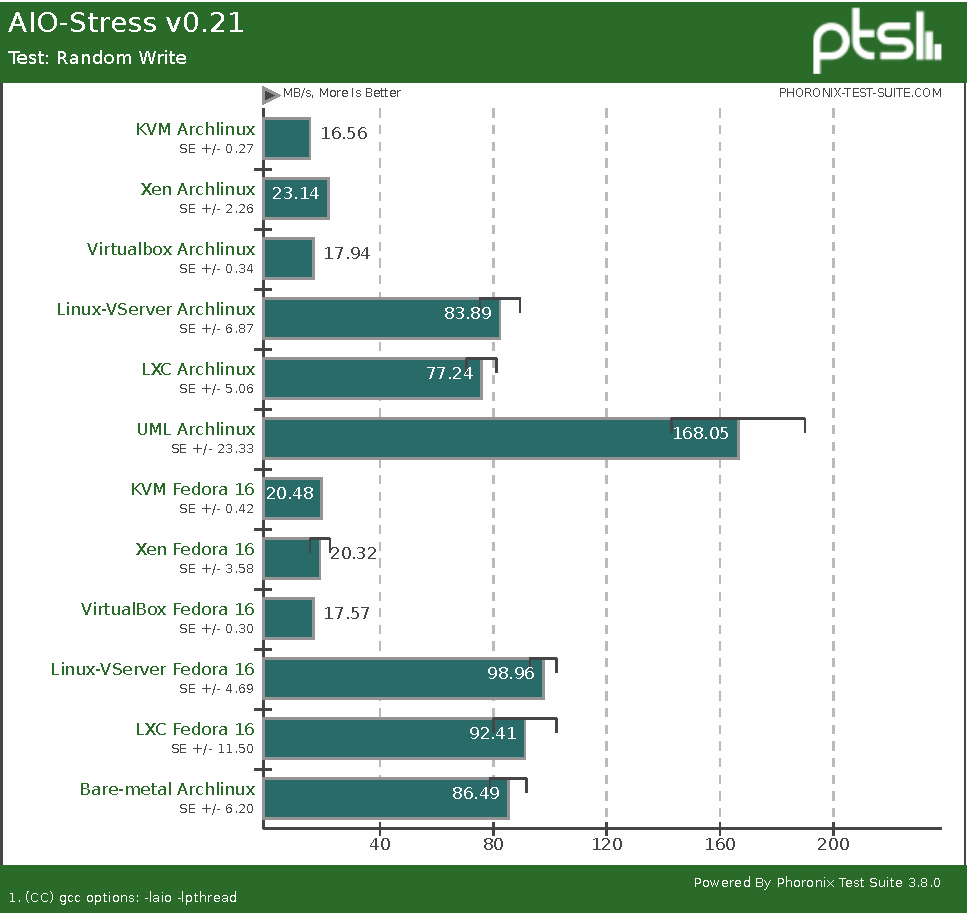
\includegraphics[width=15cm]{obr/bench/aio-stress-graph}
  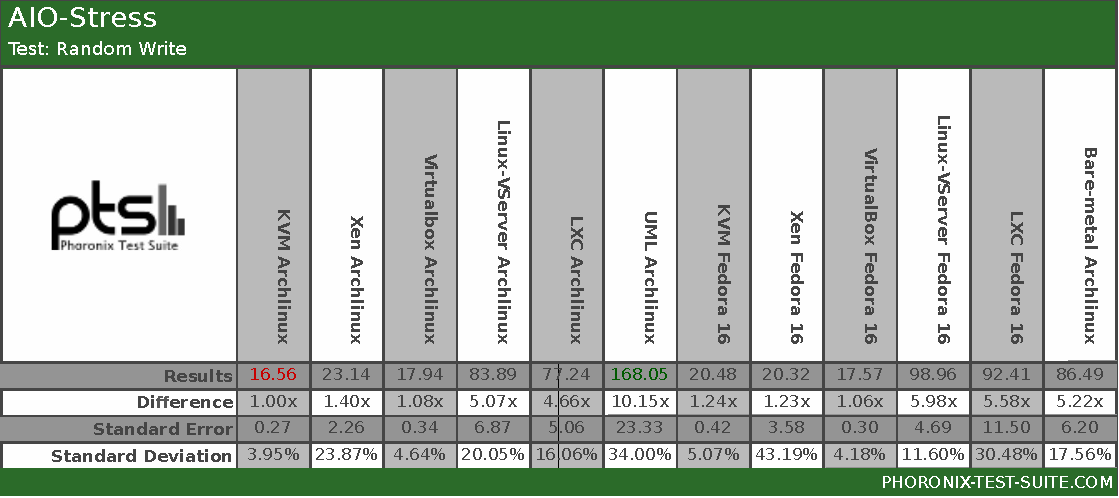
\includegraphics[width=15cm]{obr/bench/aio-stress-table}
  \caption{Výsledky AIO-Stress.}
  \label{obr:bench:aio}
\end{figure}




\begin{figure}[h!]
  \centering
  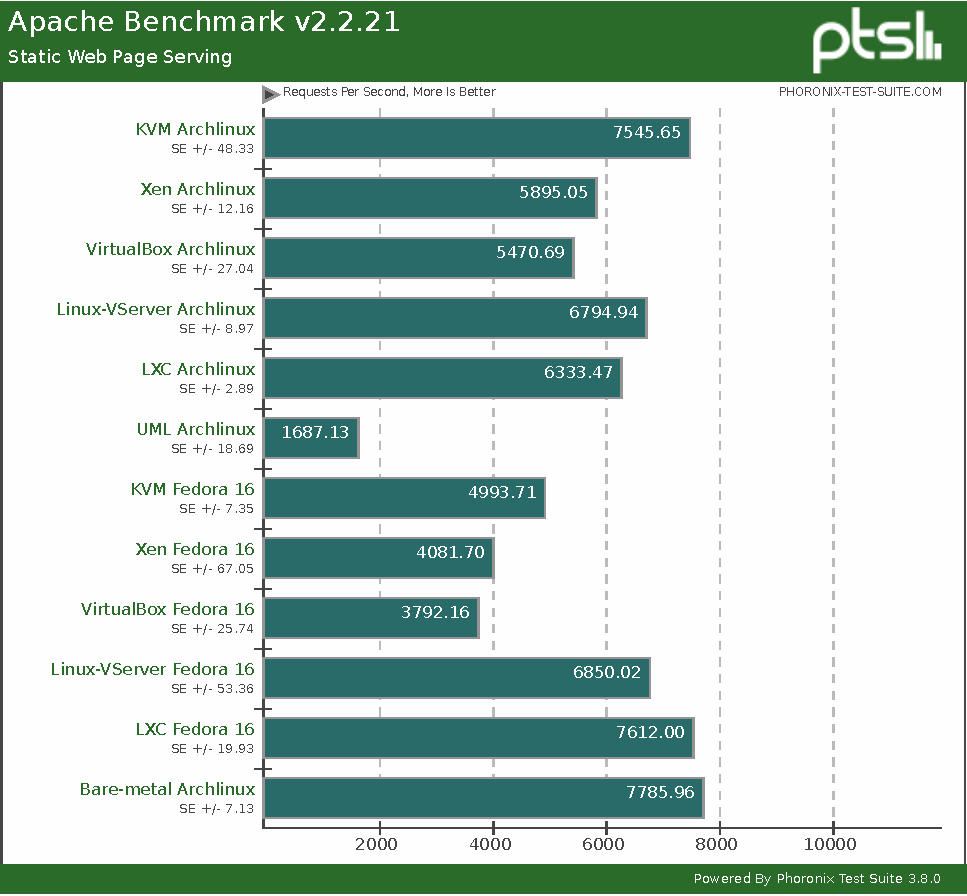
\includegraphics[width=15cm]{obr/bench/apache-graph}
  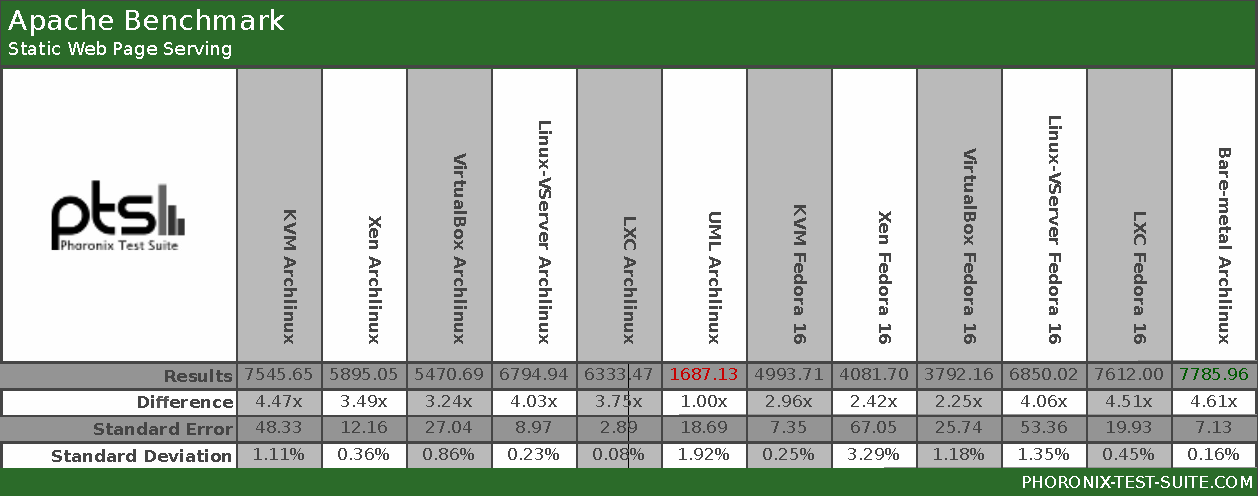
\includegraphics[width=15cm]{obr/bench/apache-table}
  \caption{Naměřené hodnoty Apache benchmarku.}
  \label{obr:bench:apache}
\end{figure}



\begin{figure}[h!]
  \centering
  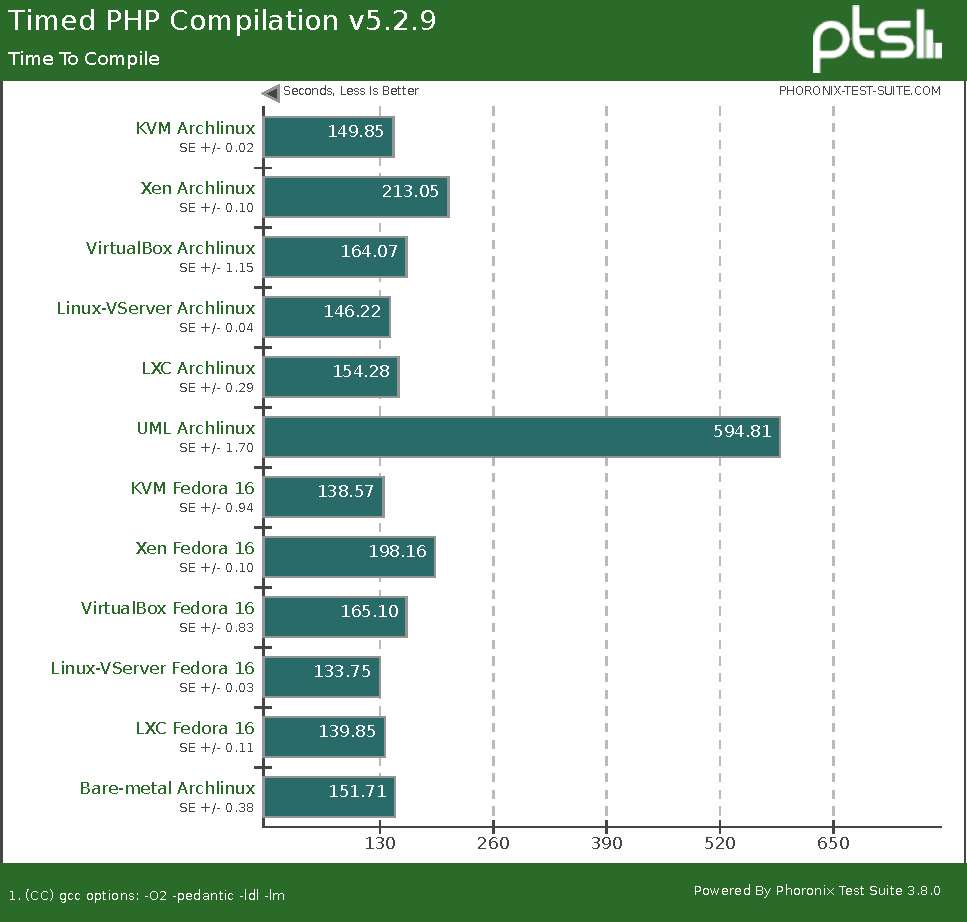
\includegraphics[width=15cm]{obr/bench/build-php-graph}
  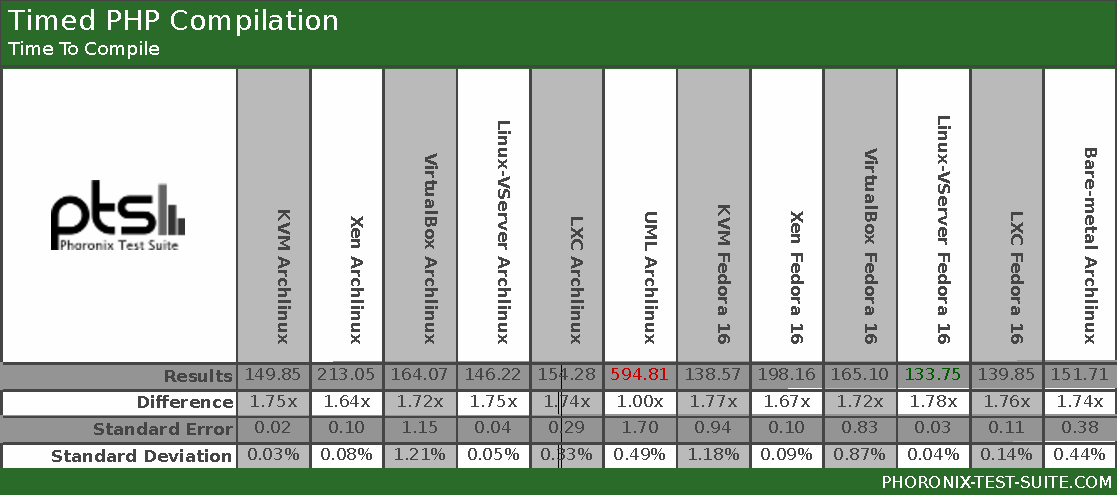
\includegraphics[width=15cm]{obr/bench/build-php-table}
  \caption{Výsledné hodnoty sestavování PHP aplikace.}
  \label{obr:bench:buildphp}
\end{figure}



\begin{figure}[h!]
  \centering
  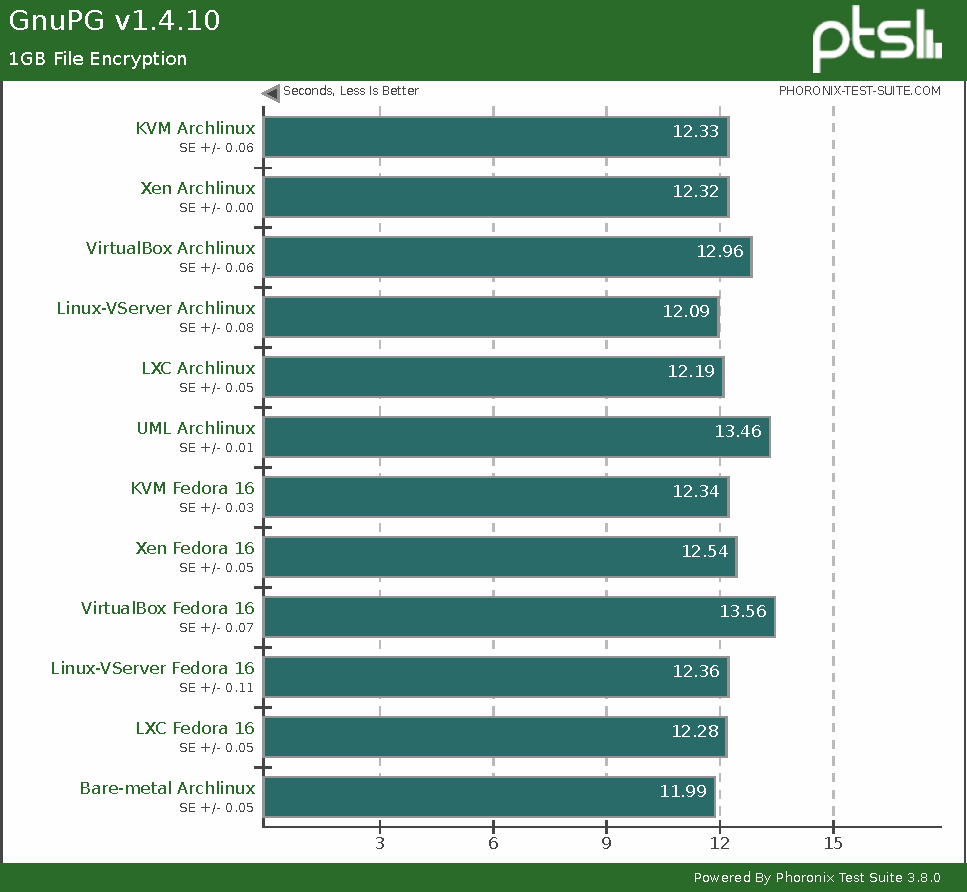
\includegraphics[width=15cm]{obr/bench/gnupg-graph}
  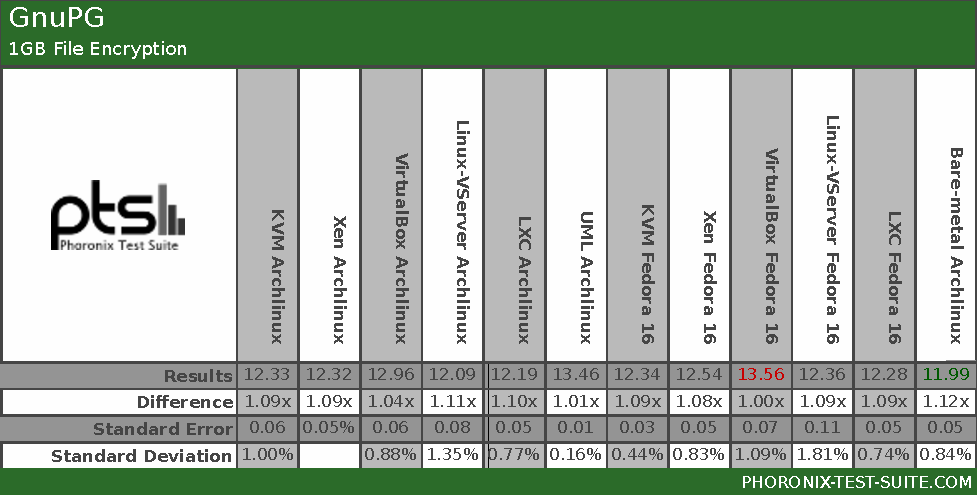
\includegraphics[width=15cm]{obr/bench/gnupg-table}
  \caption{Doba potřebná k zašifrování soubrou pomocí GnuPG.}
  \label{obr:bench:gnupg}
\end{figure}



\begin{figure}[h!]
  \centering
  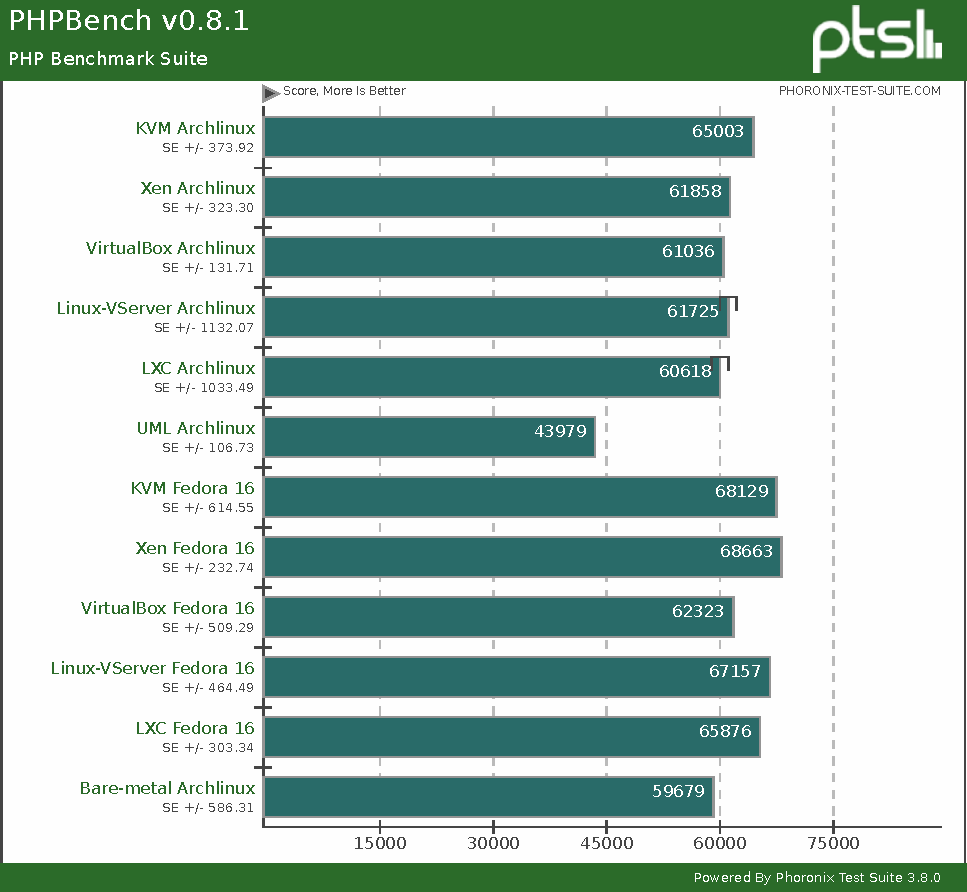
\includegraphics[width=15cm]{obr/bench/phpbench-graph}
  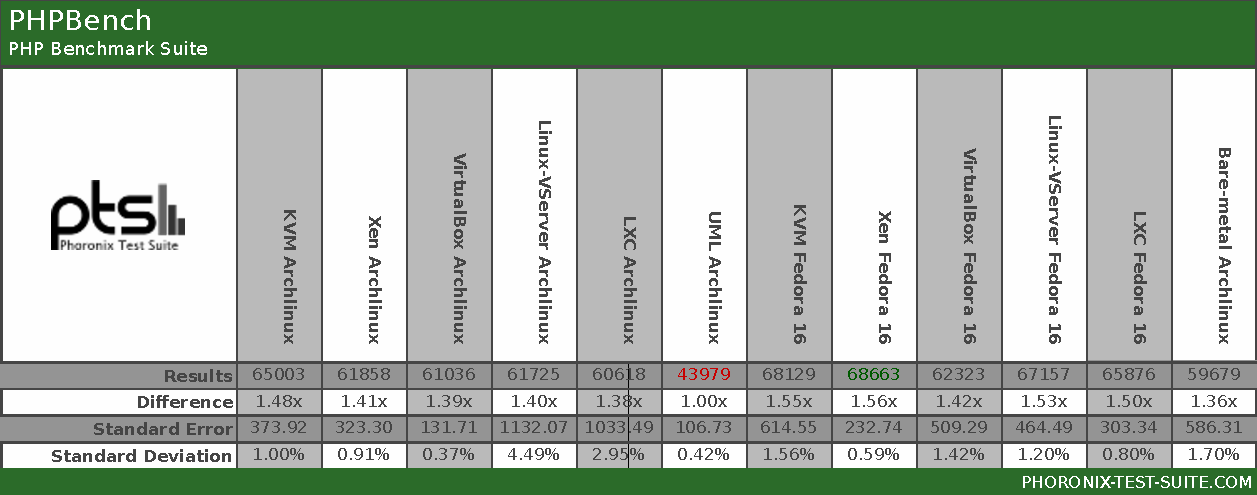
\includegraphics[width=15cm]{obr/bench/phpbench-table}
  \caption{Počet bodů získaný v PHPBench.}
  \label{obr:bench:phpbench}
\end{figure}



\begin{figure}[h!]
  \centering
  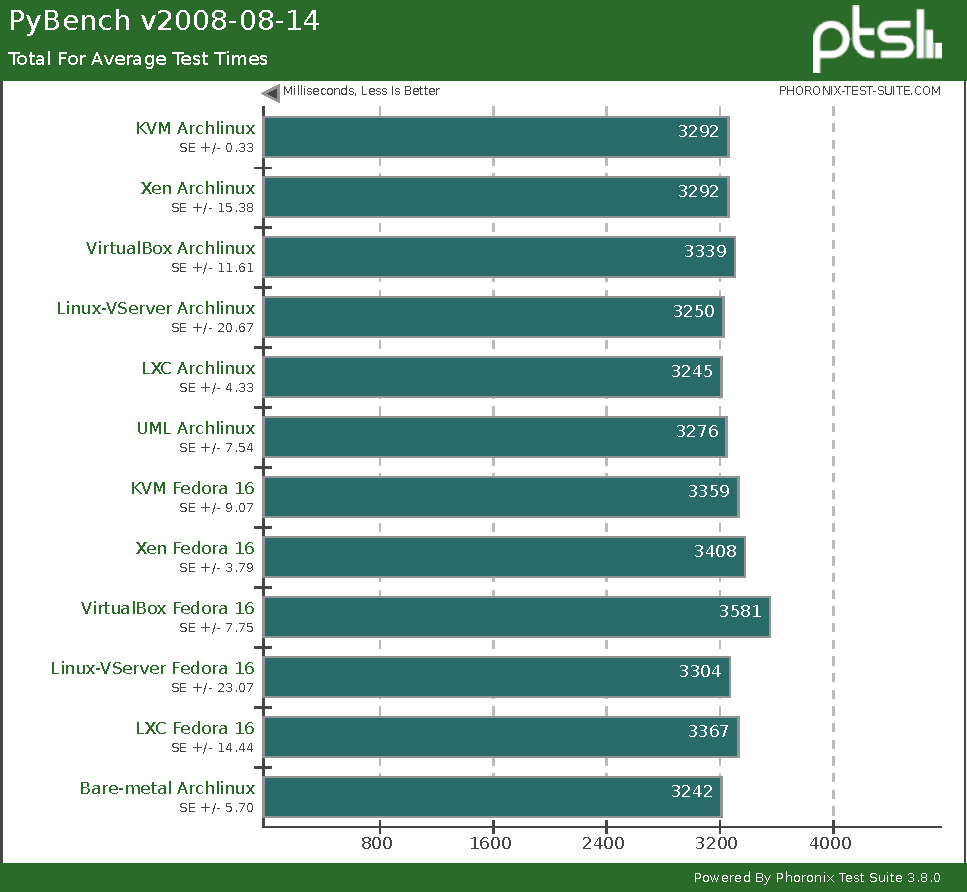
\includegraphics[width=15cm]{obr/bench/pybench-graph}
  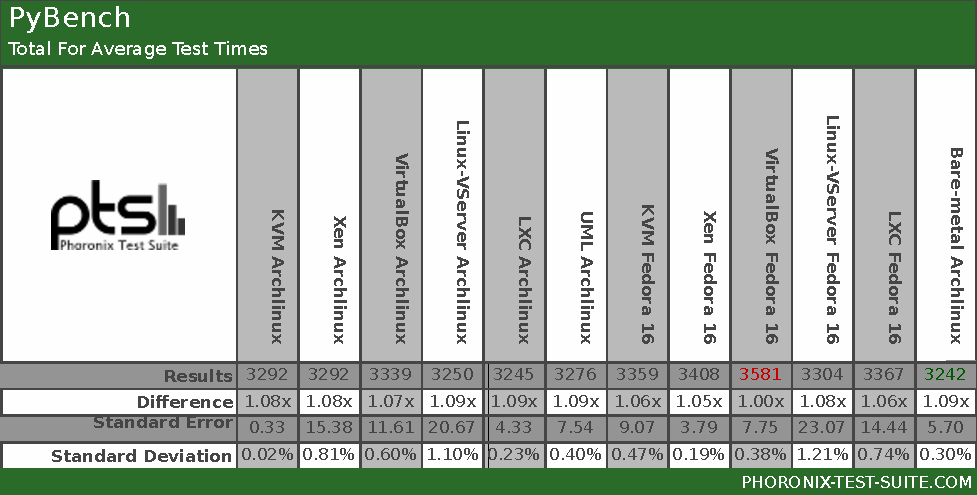
\includegraphics[width=15cm]{obr/bench/pybench-table}
  \caption{Doba nutná pro dokončení PyBench.}
  \label{obr:bench:pybench}
\end{figure}

\begin{figure}[h!]
  \centering
  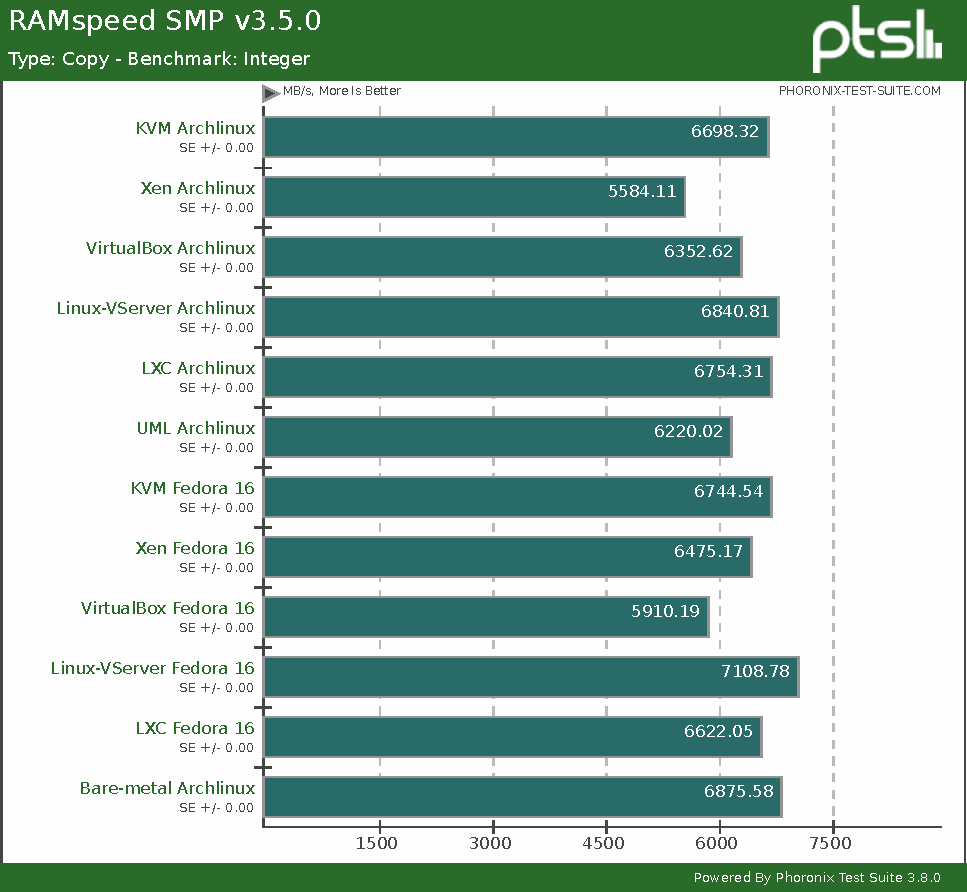
\includegraphics[width=15cm]{obr/bench/ramspeed-graph}
  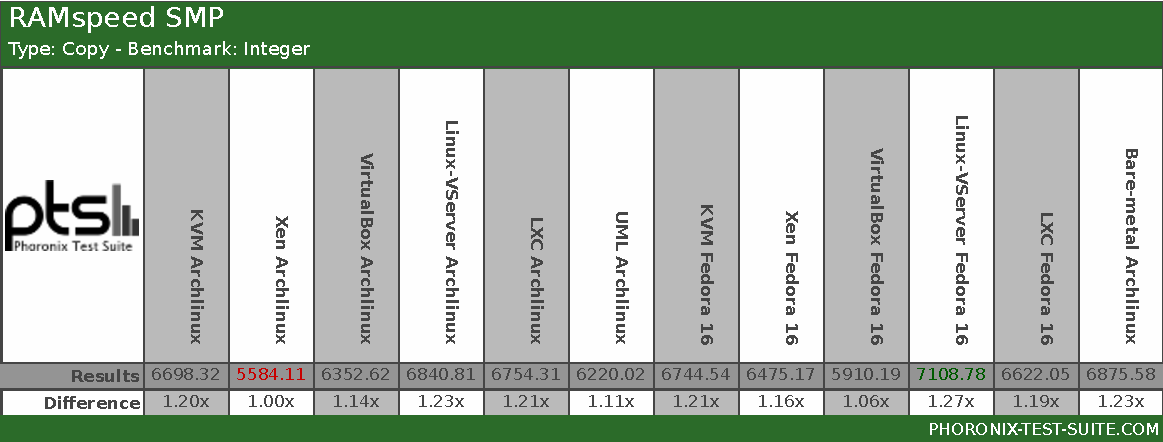
\includegraphics[width=15cm]{obr/bench/ramspeed-table}
  \caption{Rychlost kopírování celého čísla v MB/s.}
  \label{obr:bench:ramspeed}
\end{figure}



\begin{figure}[h!]
  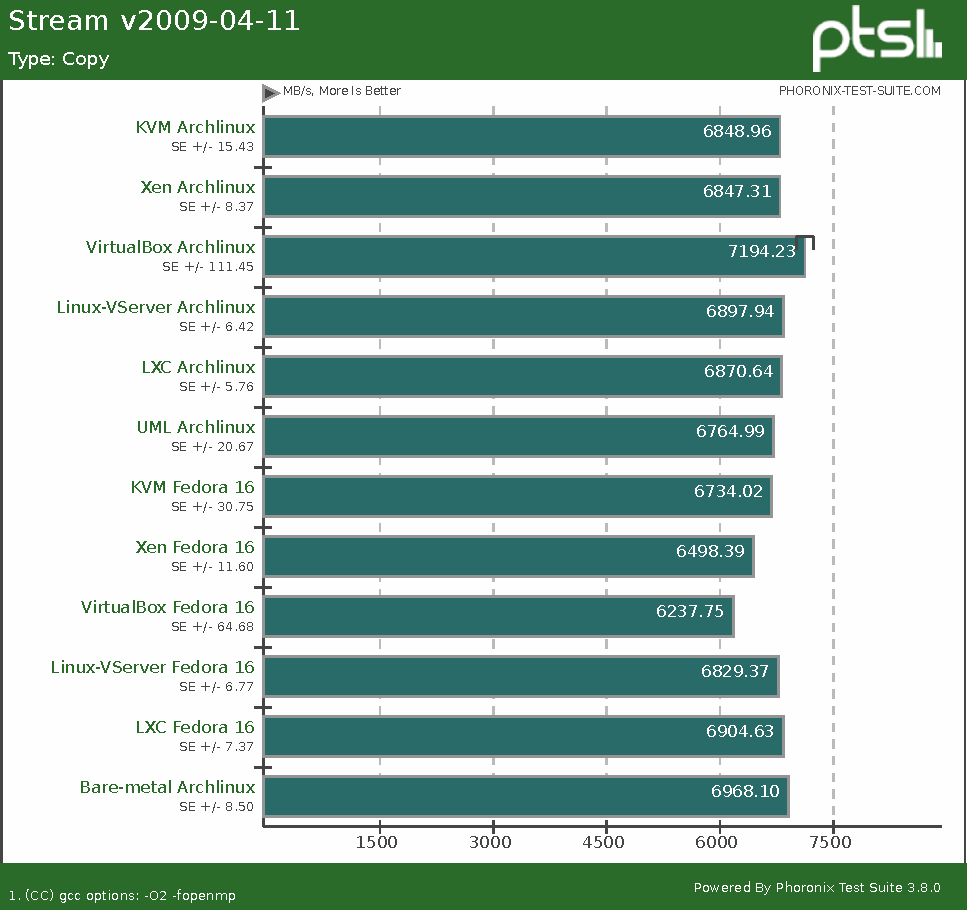
\includegraphics[width=75mm]{obr/bench/stream-graph-1}
  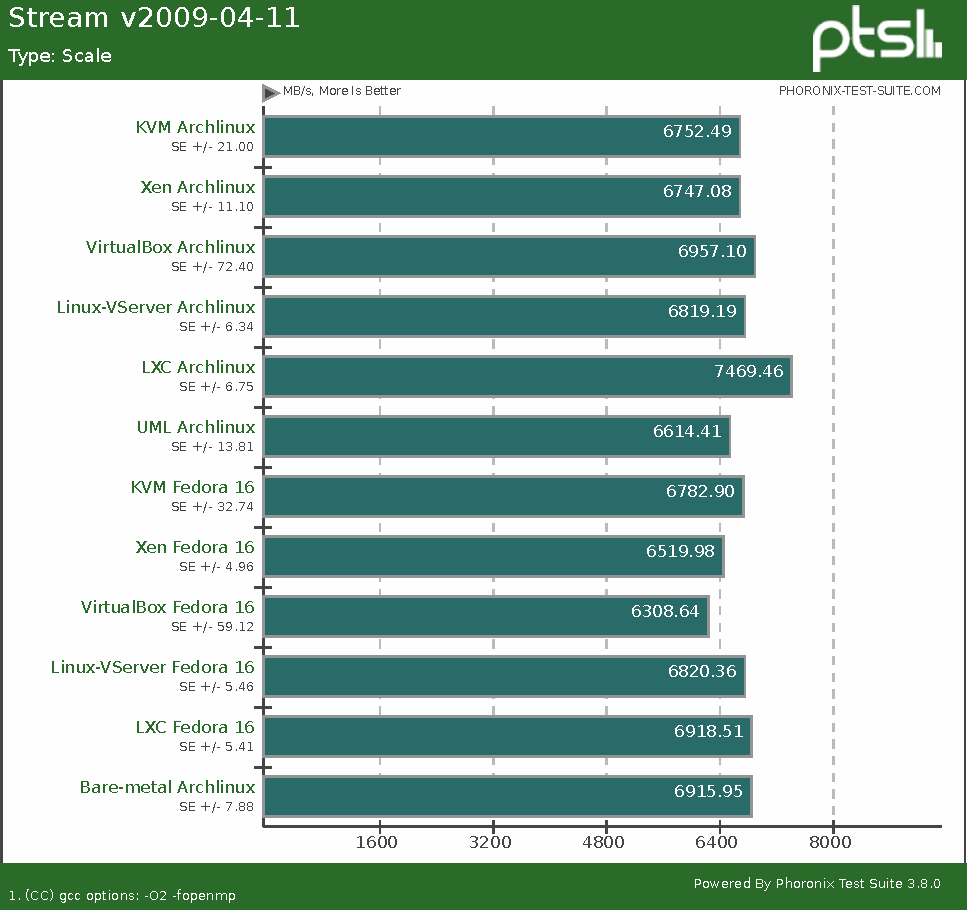
\includegraphics[width=75mm]{obr/bench/stream-graph-2}
  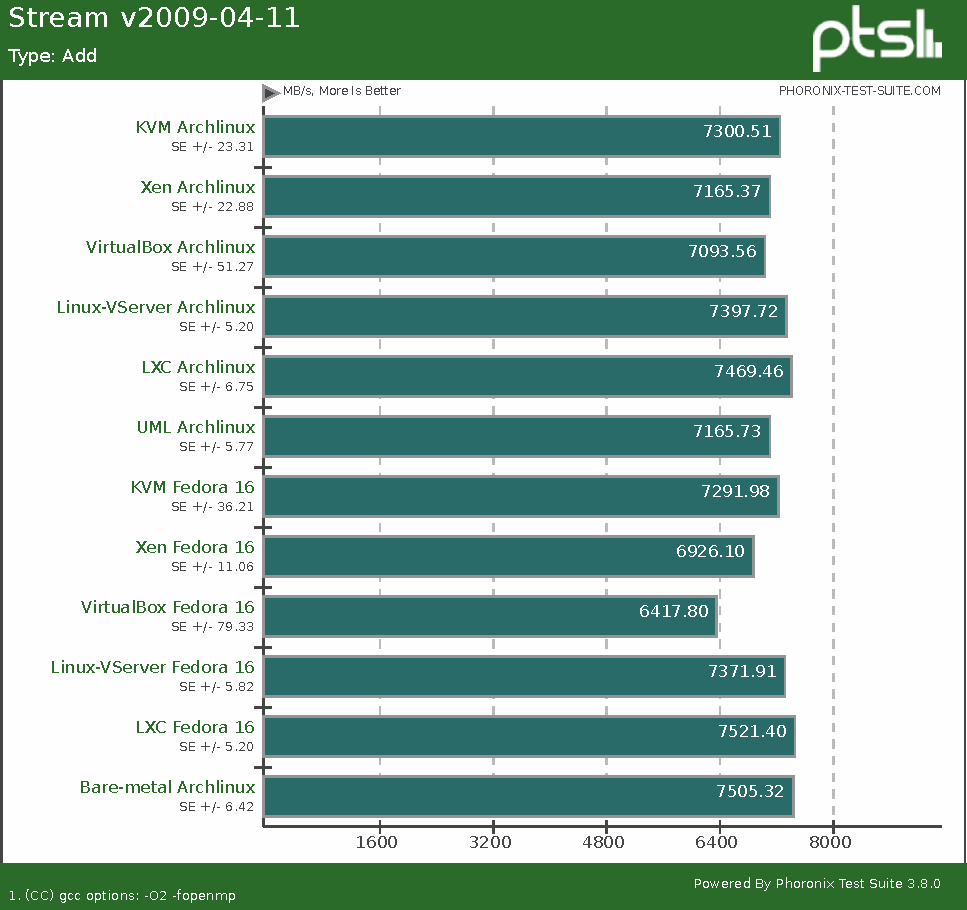
\includegraphics[width=75mm]{obr/bench/stream-graph-3}
  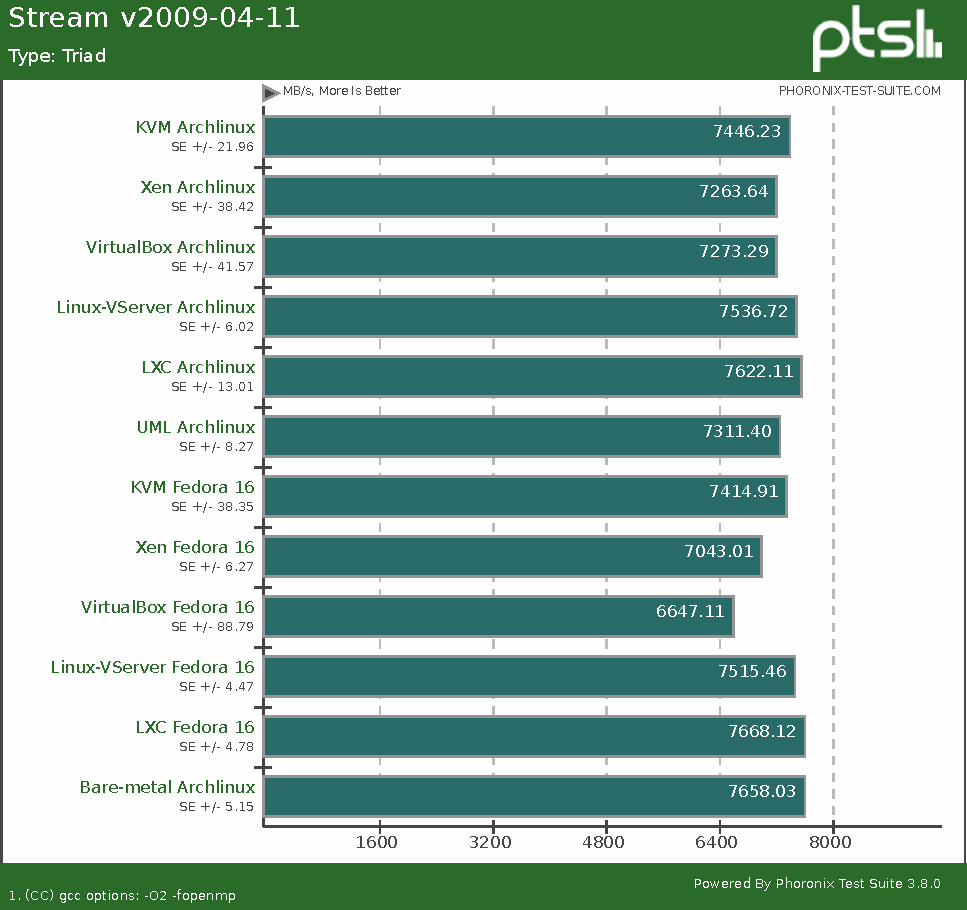
\includegraphics[width=75mm]{obr/bench/stream-graph-4}
  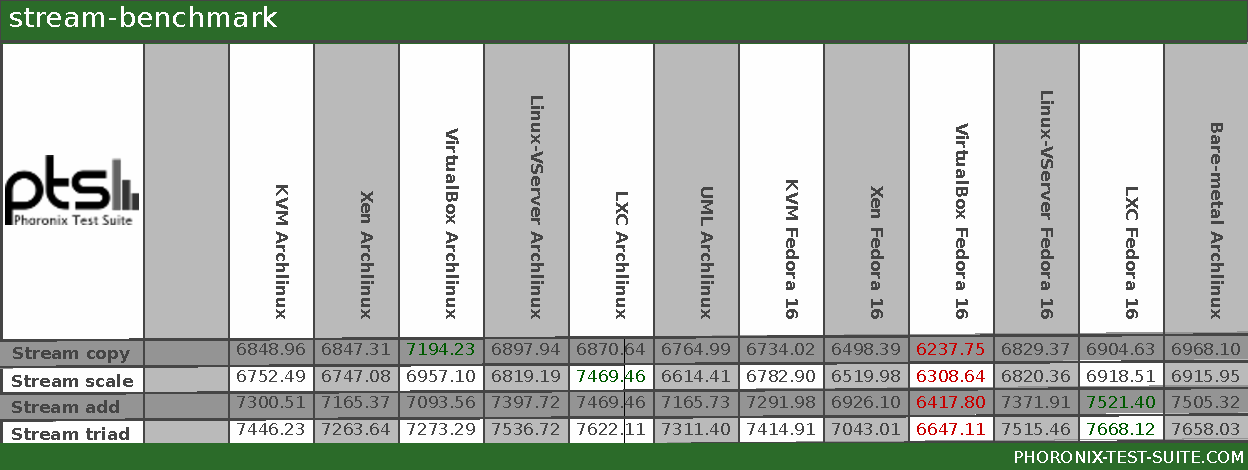
\includegraphics[width=152mm]{obr/bench/stream-table}
  \caption{Rychlost operací s operační pamětí.}
  \label{obr:bench:stream}
\end{figure}


\begin{figure}[h!]
  \centering
  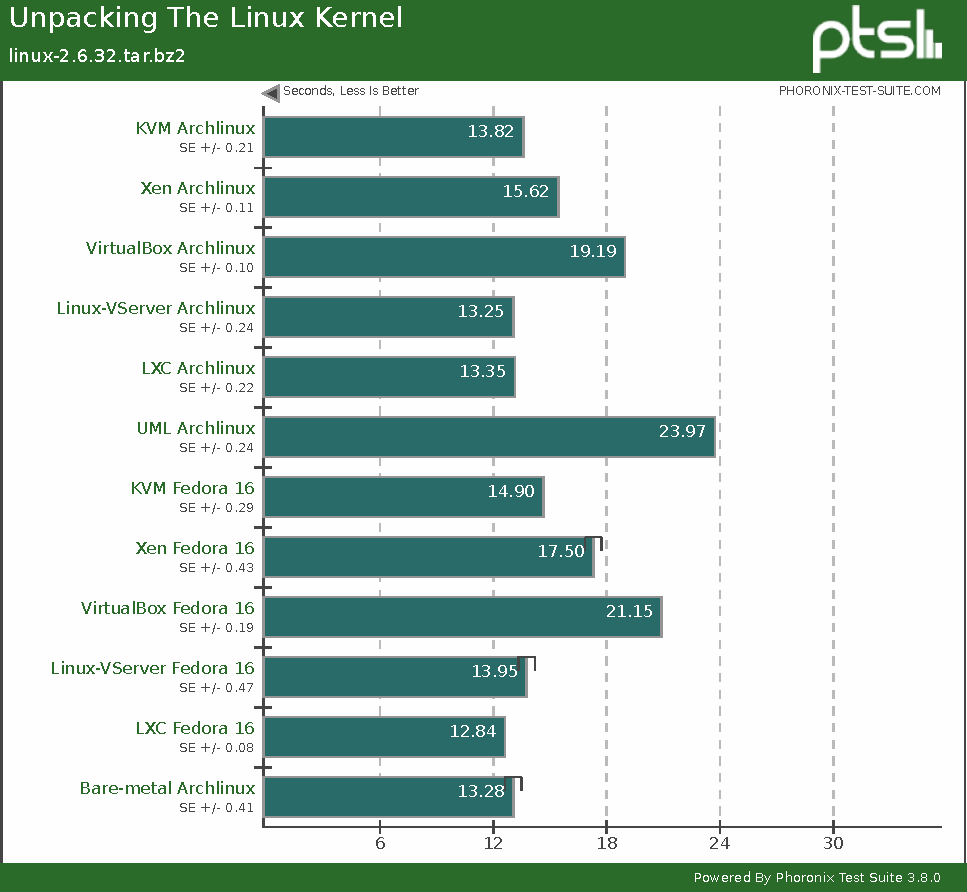
\includegraphics[width=15cm]{obr/bench/unpack-linux-graph}
  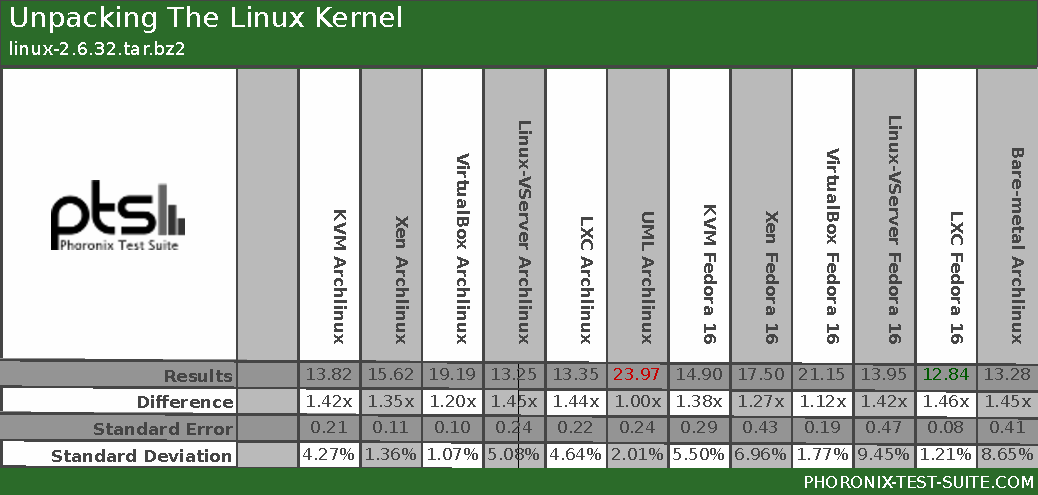
\includegraphics[width=15cm]{obr/bench/unpack-linux-table}
  \caption{Doba za jak dlouho se rozbalí zdrojové kódy jádra linuxu.}
  \label{obr:bench:unpacklinux}
\end{figure}


\begin{figure}[h!]
  \centering
  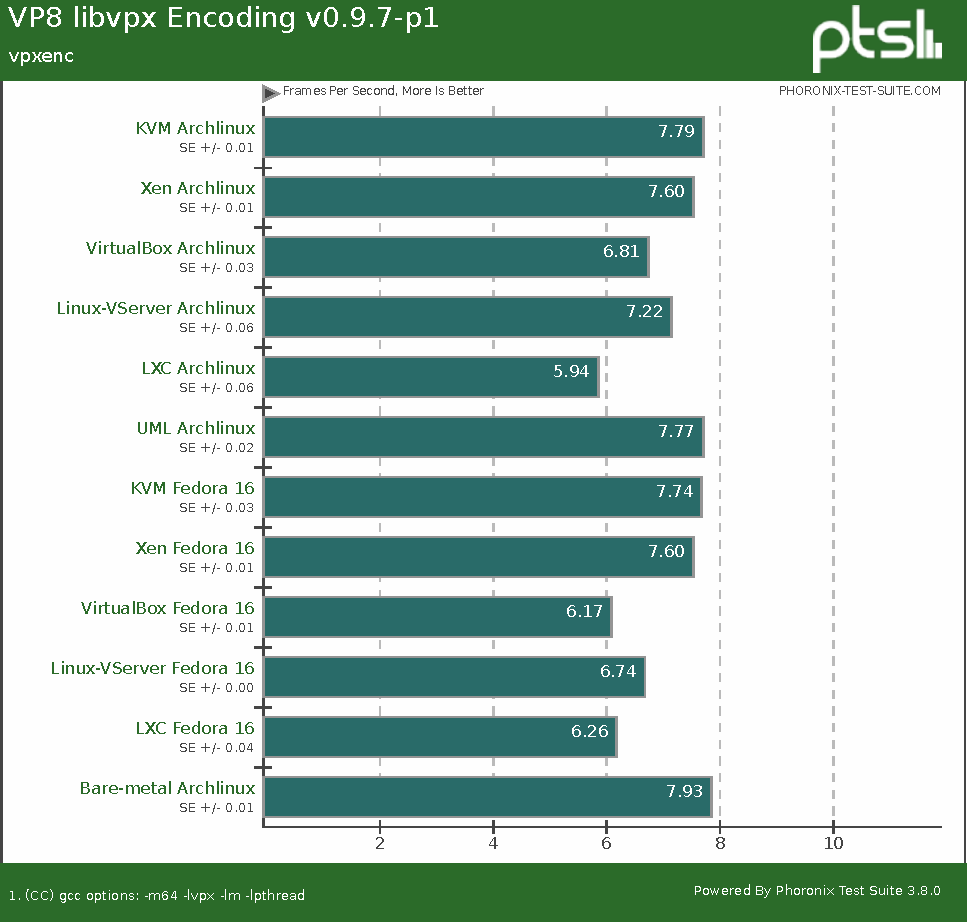
\includegraphics[width=15cm]{obr/bench/vpxenc-graph}
  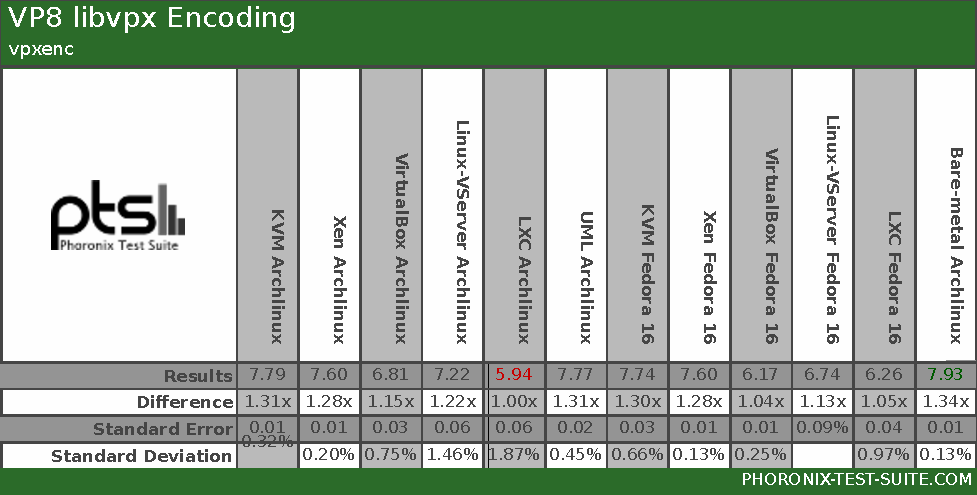
\includegraphics[width=15cm]{obr/bench/vpxenc-table}
  \caption{Počet snímků za sekundu - enkódování do VP8.}
  \label{obr:bench:vpxenc}
\end{figure}



\begin{figure}[h!]
  \centering
  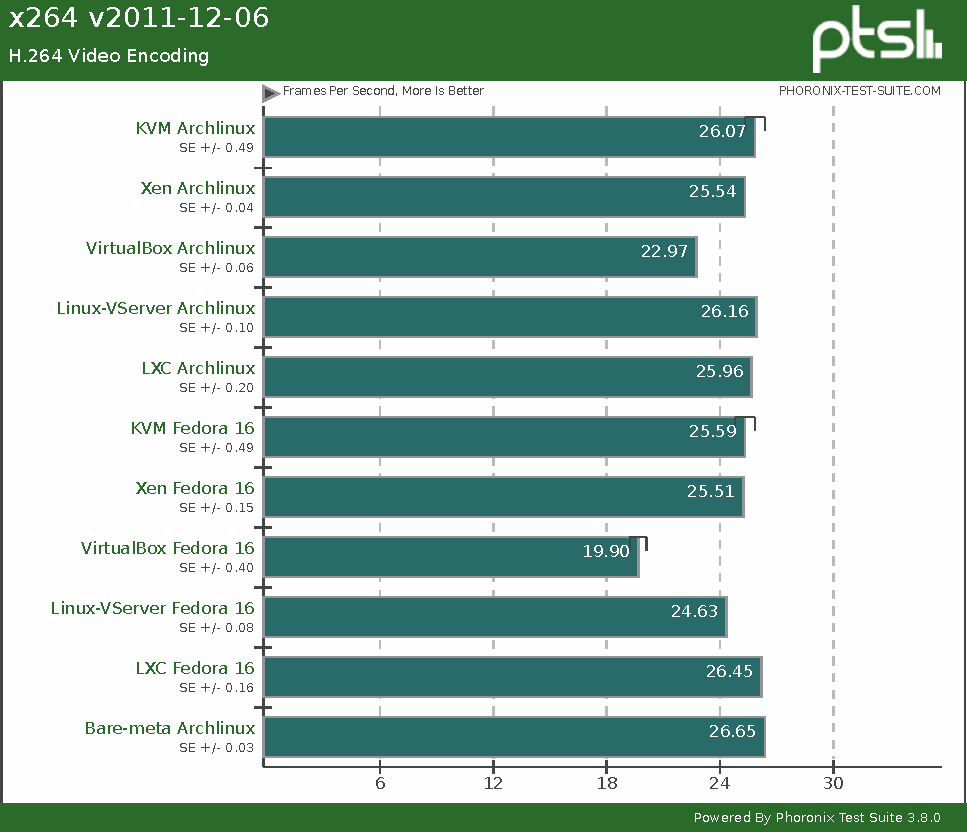
\includegraphics[width=15cm]{obr/bench/x264-graph}
  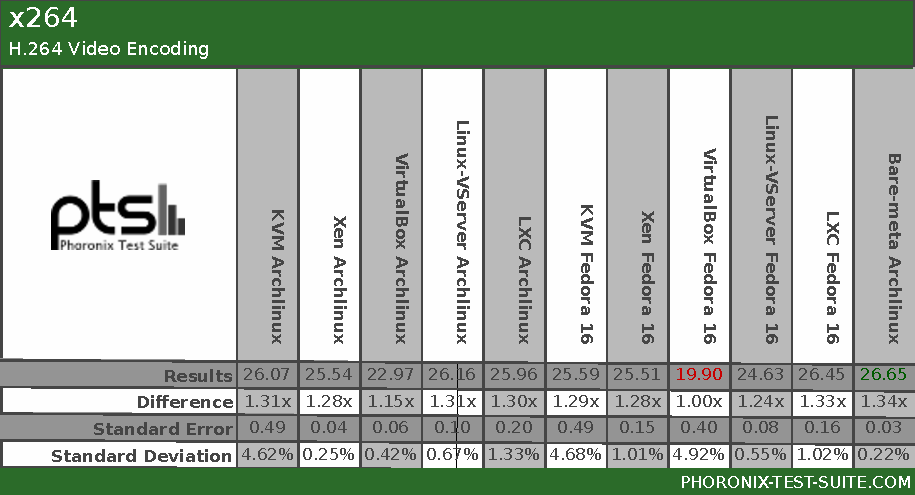
\includegraphics[width=15cm]{obr/bench/x264-table}
  \caption{Počet snímků za sekundu - enkódování do H264.}
  \label{obr:bench:x264}
\end{figure}
